\section{Scale3DMatrix Class Reference}
\label{classScale3DMatrix}\index{Scale3DMatrix@{Scale3DMatrix}}
{\tt \#include $<$scale3dmatrix.h$>$}

Inheritance diagram for Scale3DMatrix::\begin{figure}[H]
\begin{center}
\leavevmode
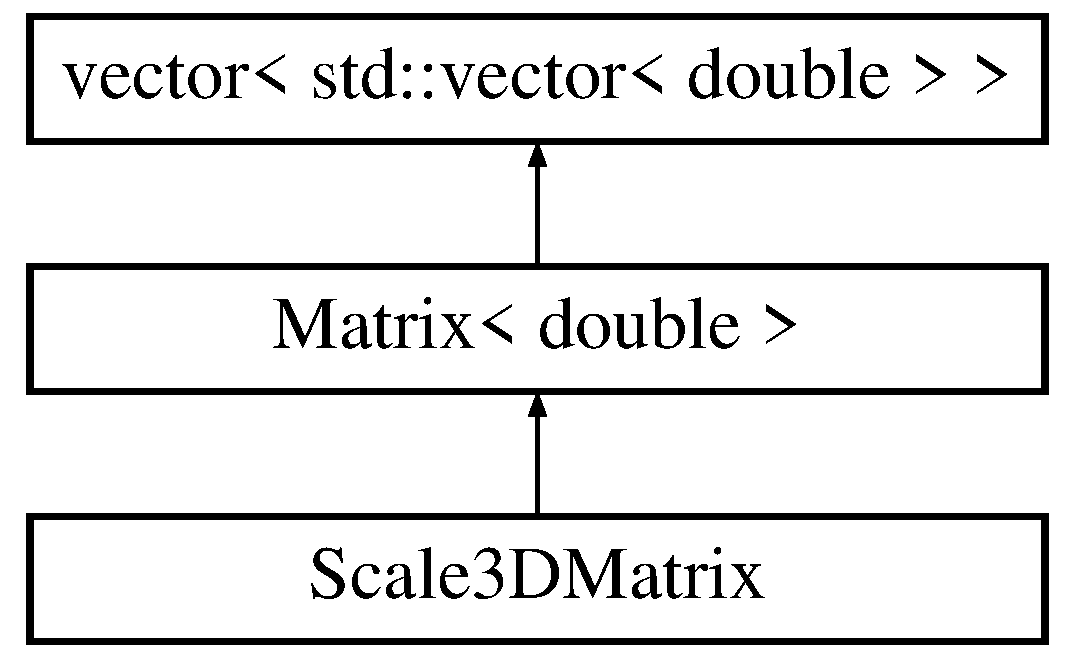
\includegraphics[height=3cm]{classScale3DMatrix}
\end{center}
\end{figure}
\subsection*{Public Methods}
\begin{CompactItemize}
\item 
{\bf Scale3DMatrix} (double x\-Scale, double y\-Scale, double z\-Scale)
\item 
{\bf Scale3DMatrix} (double scale)
\end{CompactItemize}


\subsection{Constructor \& Destructor Documentation}
\index{Scale3DMatrix@{Scale3DMatrix}!Scale3DMatrix@{Scale3DMatrix}}
\index{Scale3DMatrix@{Scale3DMatrix}!Scale3DMatrix@{Scale3DMatrix}}
\subsubsection{\setlength{\rightskip}{0pt plus 5cm}Scale3DMatrix::Scale3DMatrix (double {\em x\-Scale}, double {\em y\-Scale}, double {\em z\-Scale})\hspace{0.3cm}{\tt  [inline]}}\label{classScale3DMatrix_a0}


\index{Scale3DMatrix@{Scale3DMatrix}!Scale3DMatrix@{Scale3DMatrix}}
\index{Scale3DMatrix@{Scale3DMatrix}!Scale3DMatrix@{Scale3DMatrix}}
\subsubsection{\setlength{\rightskip}{0pt plus 5cm}Scale3DMatrix::Scale3DMatrix (double {\em scale})\hspace{0.3cm}{\tt  [inline]}}\label{classScale3DMatrix_a1}




The documentation for this class was generated from the following file:\begin{CompactItemize}
\item 
{\bf scale3dmatrix.h}\end{CompactItemize}
